\documentclass[12pt]{article}


\author{Daniel Eberharter\\ Claudio Canella}
\title{Ridge regression}

\usepackage{amsmath}
\usepackage{graphicx}


\begin{document}
\maketitle


\section{Algorithmic choices}
Our method does not substantially differ from the one discussed in class. We chose two non-linear functions, one is $f(x) = x^2 + 2x + 2$ and the other one is $f(x) = 6x^2 + 2x + 2$. We then compute $r^t(x) = f(x^t) + \epsilon$, where $\epsilon$ is drawn from a standard uniform distribution(in octave calculated by stdnormal\_pdf) with a random error selected between 0 and 15 weighted by the variance(for full information on calculation please see code). With this function we calculate our training- and validation set. We calculate our design matrix and use the formula that has been introduced in the lecture to calculate our regression coefficients for each $\lambda$ and to avoid biasing towards $w_0$ we center our values. By using M-fold cross-validation we find our best $\lambda$.


\section{numbers and illustrations}
	\begin{itemize} \label{plotted}
		\item x = 0 to 9
		\item N = 20
		\item M = 3
		\item probability of error: 0.15 (used for $\epsilon$)
		\item $\lambda$ = 19 generated logarithmic  values between 0 and $10^6$\\
		\item $\lambda$ plotted = least error, index of lambda at position $1+(index\_best - \frac{num\_lambda}{2}) \%\ num\_lambda$, index of lambda at position $num\_lambda -( 1+(index\_best - \frac{num\_lambda}{2}) \%\ num\_lambda)$
	\end{itemize}

	\begin{figure}
		\centering
		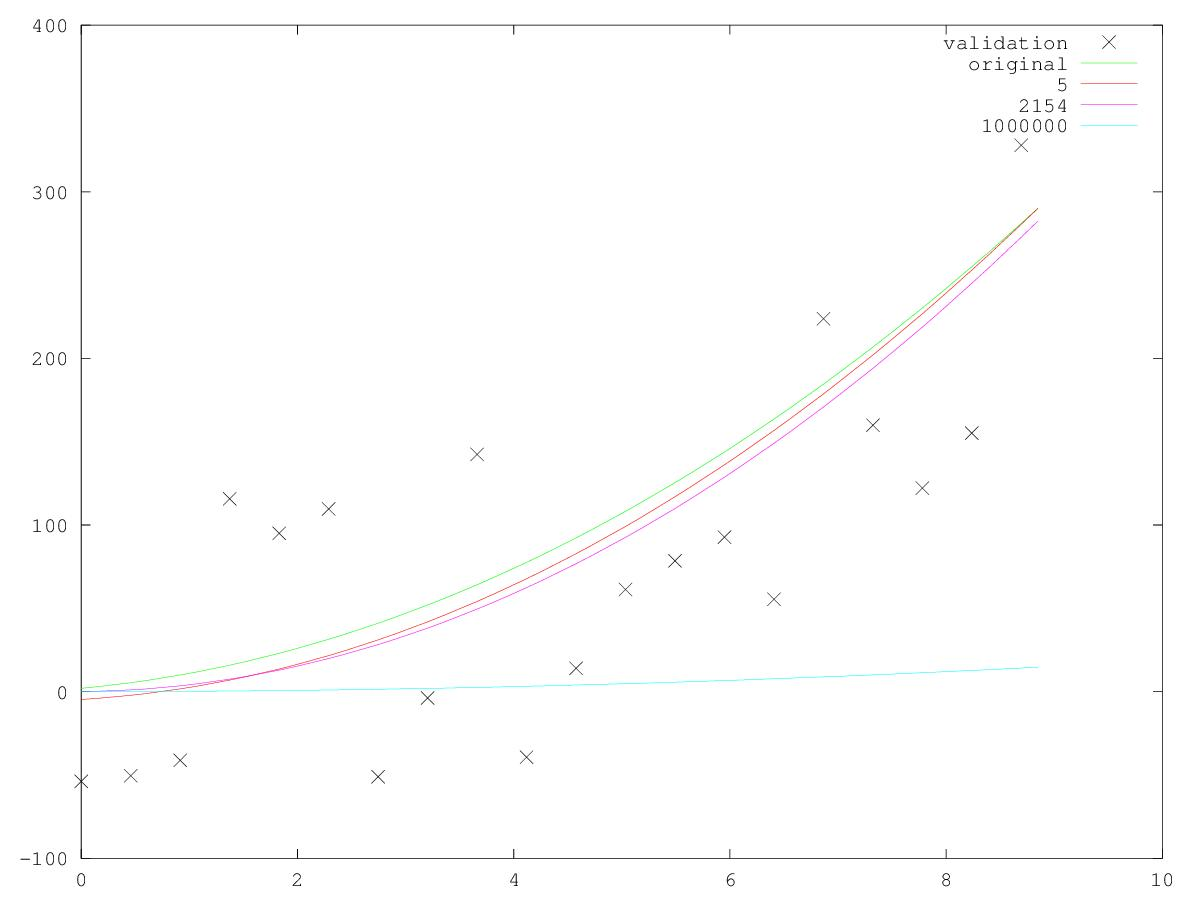
\includegraphics[scale=0.8]{plot}
		\caption{plotted graph with $\lambda$ values specified as in list \ref{plotted}}
	\end{figure}
\\
As it is part of the task, we created a plot with $\lambda$ on the abscissa and the error on the ordinateas it can be seen in figures \ref{log_1} and \ref{log_2}. 

In figures  we can see all the calculated errors for both functions with the best one being indicated as it is written to the console.

	\begin{figure}
		\centering
		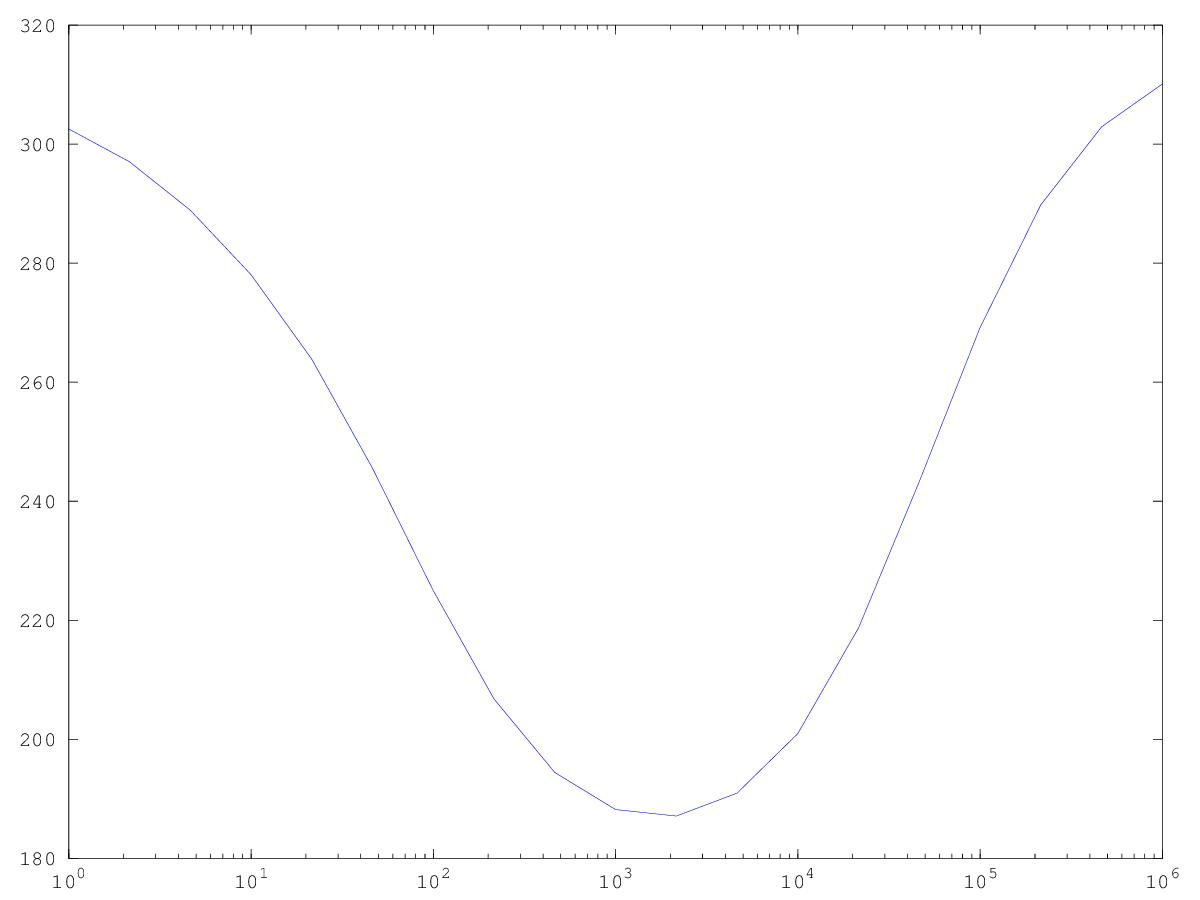
\includegraphics[scale=0.7]{log}
		\caption{ $\lambda$ and the error plotted on a logarithmic abscissa for $f(x) = 3x^2 + 6x + 2$}
		\label{log_1}
	\end{figure}
	\begin{figure}
		\centering
		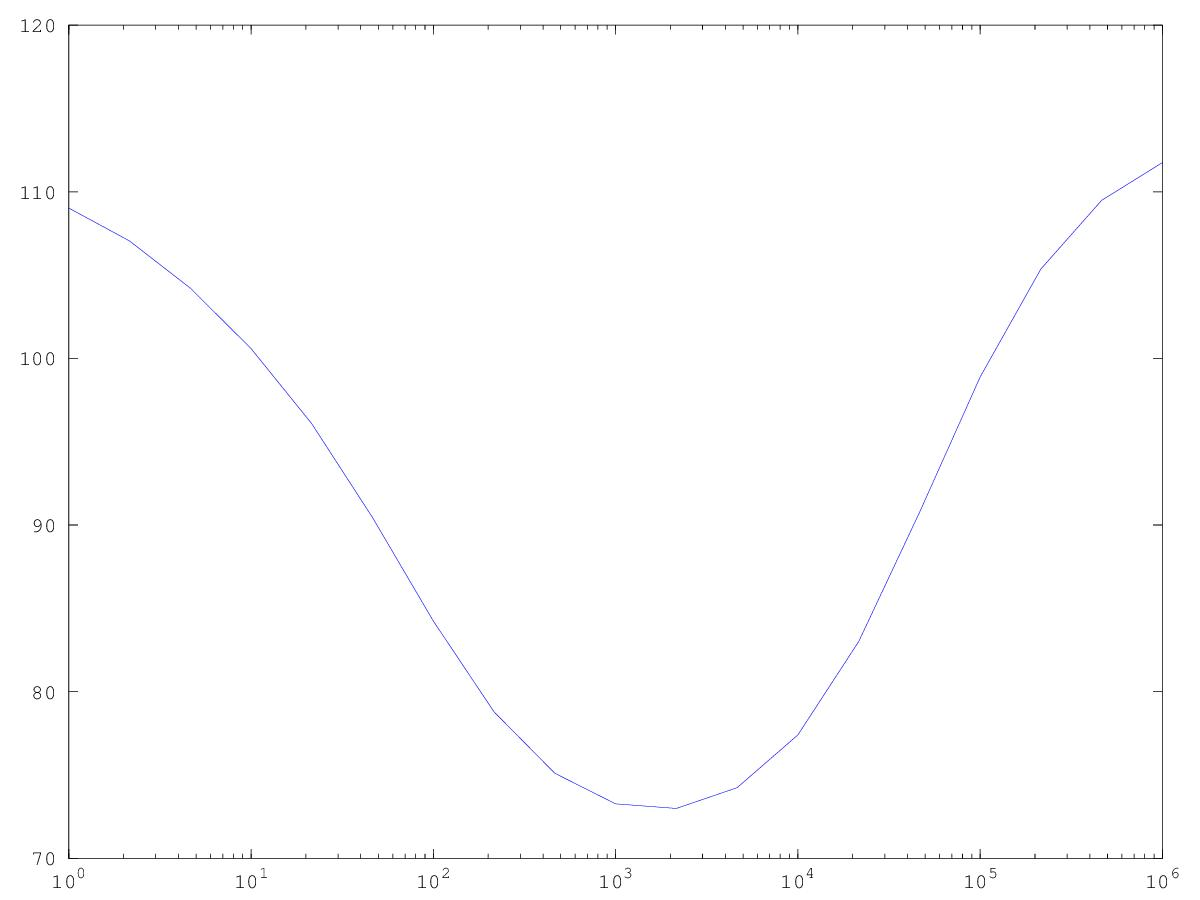
\includegraphics[scale=0.7]{log_small_f}
		\caption{ $\lambda$ and the error plotted on a logarithmic abscissa for $f(x) = x^2 + 2x + 2$}
		\label{log_2}
	\end{figure}
	
	\begin{figure}
		\centering
		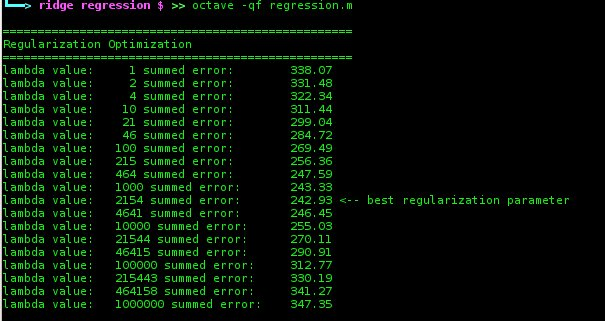
\includegraphics[scale=0.7]{console_output_big_f}
		\caption{ $\lambda$ and the error for $f(x) = 3x^2 + 6x + 2$}
		\label{log_1}
	\end{figure}
	\begin{figure}
		\centering
		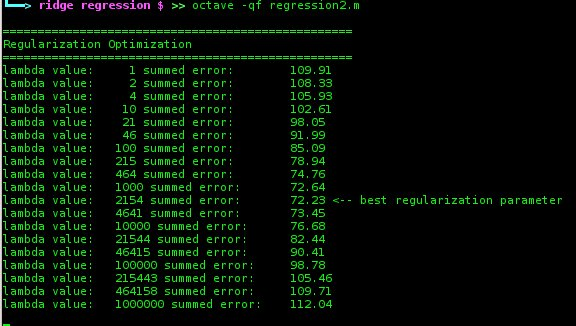
\includegraphics[scale=0.7]{console_output_small_f}
		\caption{ $\lambda$ and the error for $f(x) = x^2 + 2x + 2$}
		\label{log_2}
	\end{figure}

\section{Conclusions}
We tested our implementation with different functions without increasing the order of our polynomial as we would have to change the whole implementation of the program. Instead we increased and decreased the weighting factor of each order and our $\lambda$ values. While doing this we noticed that for the function with the higher slope($f(x) = 3x^2 + 6x + 2$) our approximation with the different $\lambda$ values is almost identical at the start, but at the end the diverge as seen in figure \ref{fig:plot}. When we use the function with the lower slope($f(x) = x^2 + 2x + 2$) it is the other way around, meaning that the approximation with the different $\lambda$ values diverge at the beginning and converge at the end as seen in figure \ref{fig:small_f_plot}.


	\begin{figure}[h]
		\centering
		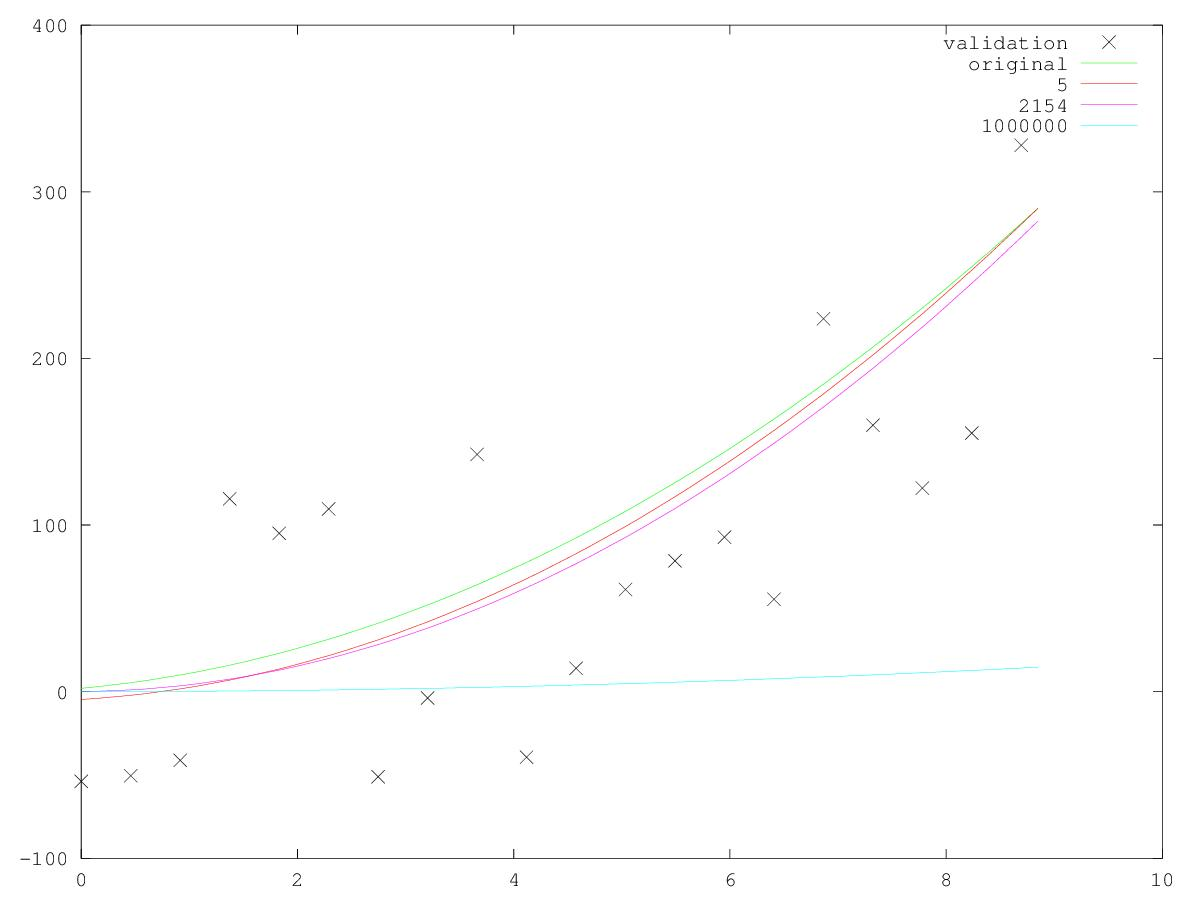
\includegraphics[scale=0.7]{plot}
		\caption{$f(x) = 3x^2 + 6x + 2$}
		\label{fig:plot}
	\end{figure}
	\begin{figure}
		\centering
		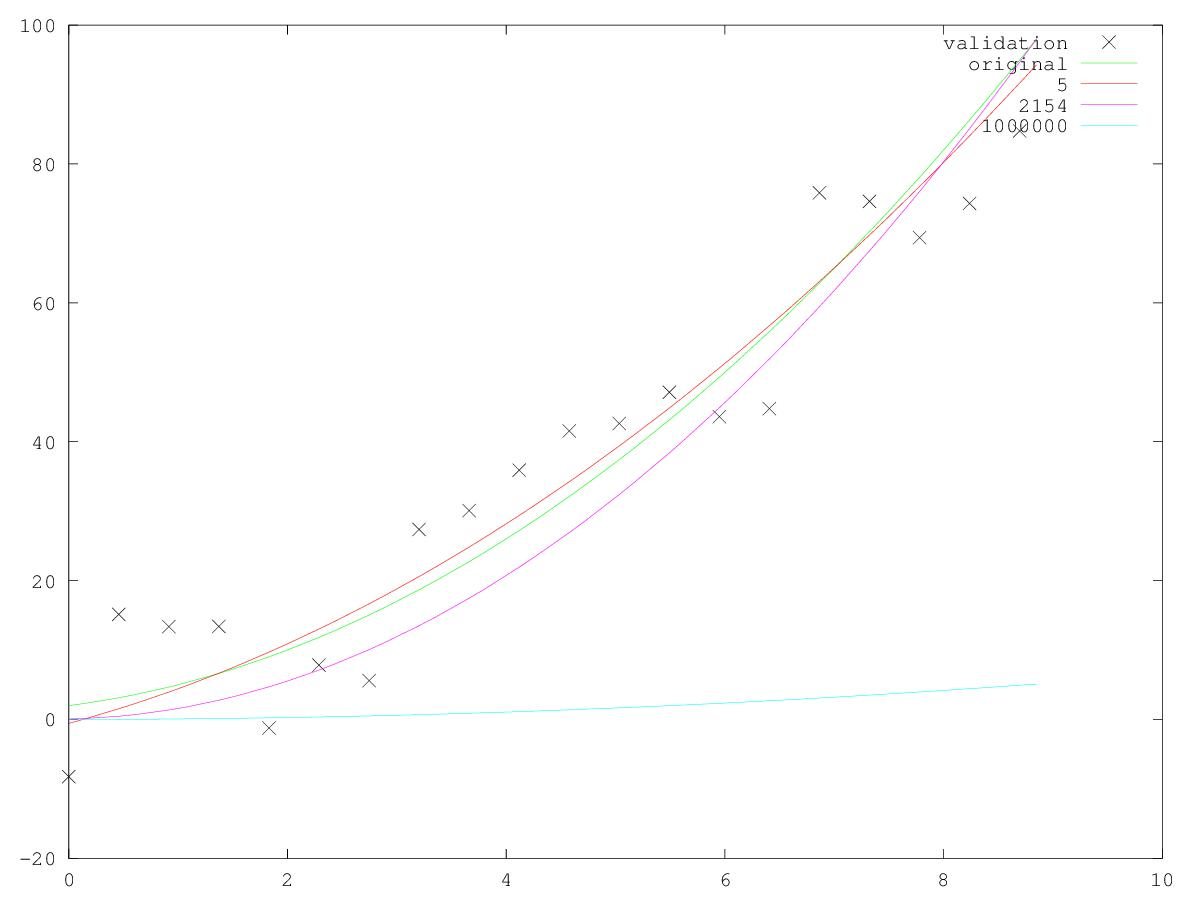
\includegraphics[scale=0.7]{small_f_plot}
		\caption{Plot for $f(x) = x^2 + 2x + 2$}
		\label{fig:small_f_plot}
	\end{figure}
\end{document}